\section{RRTExt\-Con  Class Reference}
\label{classRRTExtCon}\index{RRTExtCon@{RRTExt\-Con}}
Use Connect instead of Extend to connect the two trees. 


{\tt \#include $<$rrt.h$>$}

Inheritance diagram for RRTExt\-Con::\begin{figure}[H]
\begin{center}
\leavevmode
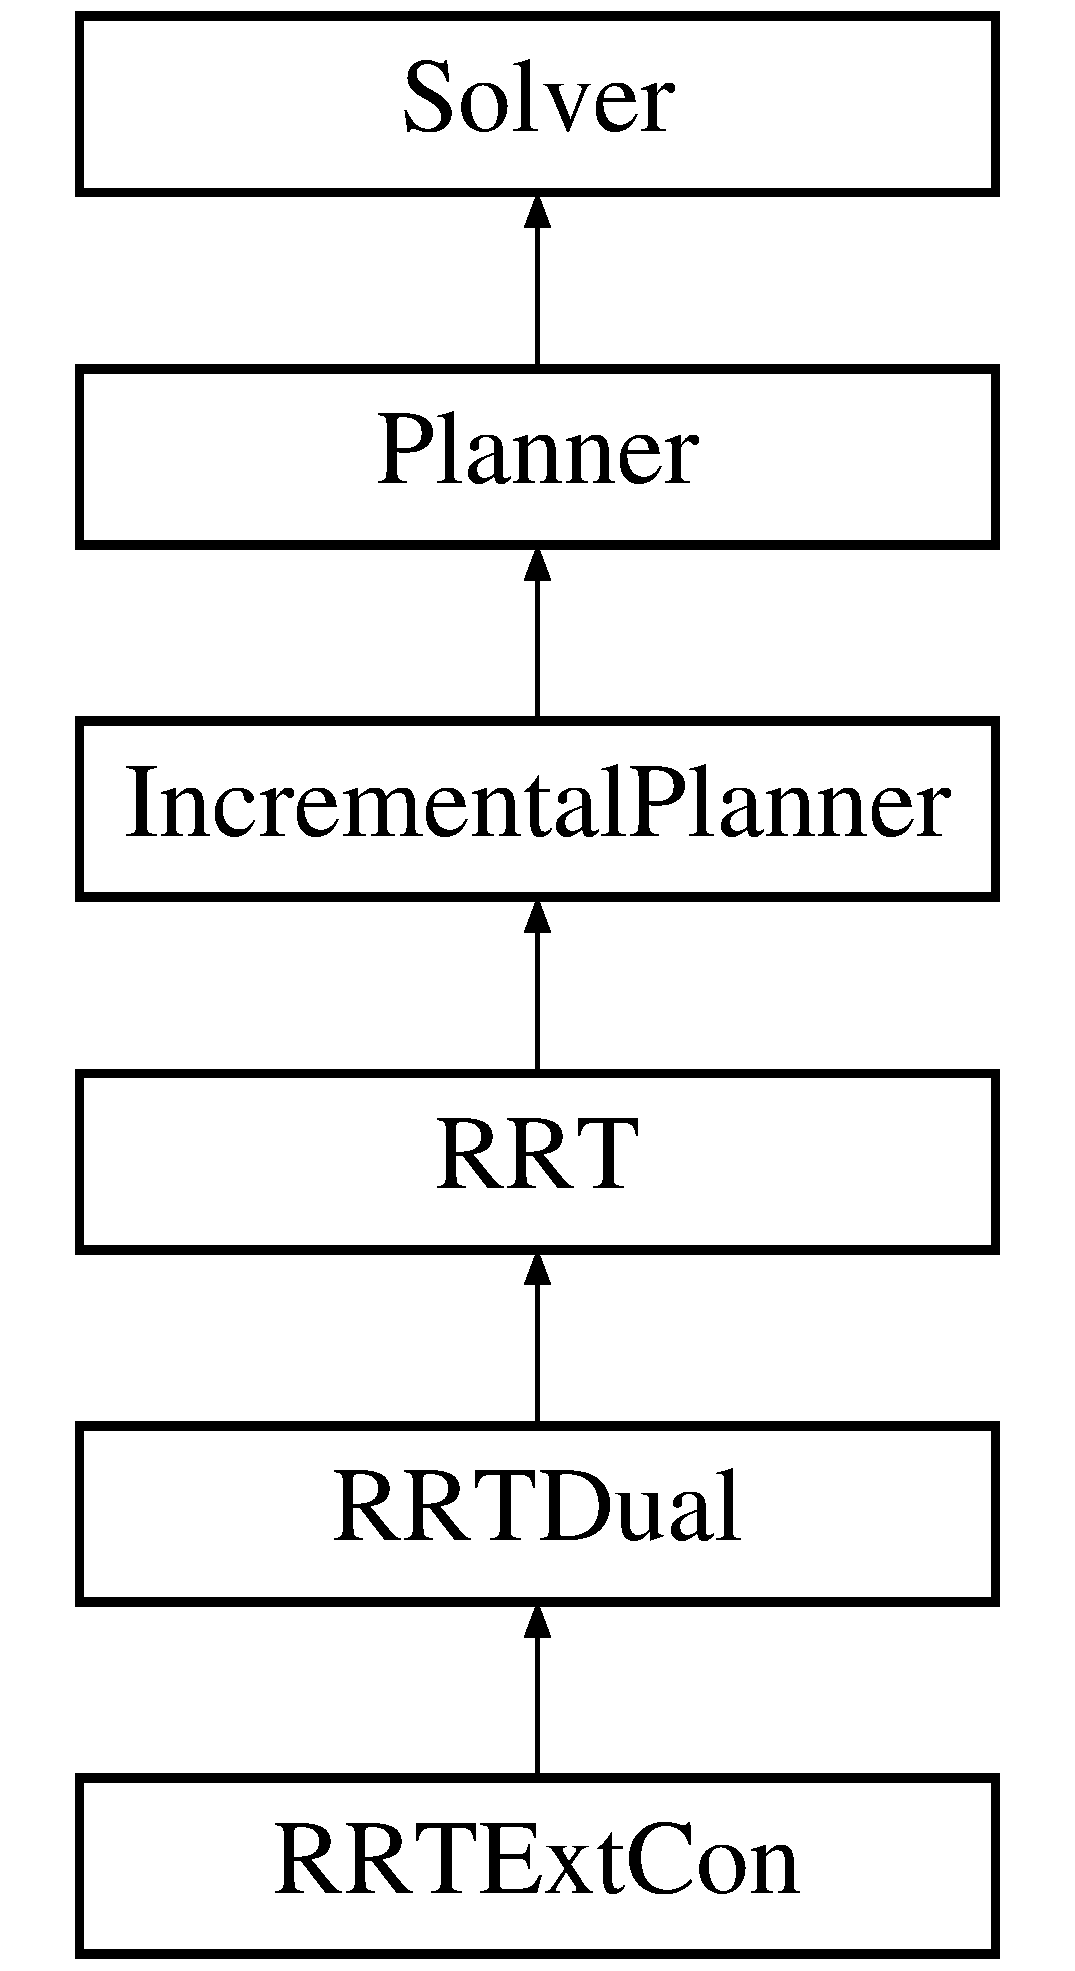
\includegraphics[height=6cm]{classRRTExtCon}
\end{center}
\end{figure}
\subsection*{Public Methods}
\begin{CompactItemize}
\item 
{\bf RRTExt\-Con} ({\bf Problem} $\ast$p)
\item 
virtual {\bf $\sim$RRTExt\-Con} ()
\item 
virtual bool {\bf Plan} ()
\begin{CompactList}\small\item\em This planner is greedier in its attempt to connect the trees.\item\end{CompactList}\end{CompactItemize}


\subsection{Detailed Description}
Use Connect instead of Extend to connect the two trees.

This planner balances the computation between growing the trees toward random samples and toward each other. G is the tree from the initial state, and G2 is the tree from the goal state. In each iteration, there are four steps: \begin{enumerate}
\item 
Use Extend to grow G toward a random sample \item 
Use Connect to grow G2 toward the new node in G \item 
Use Extend to grow G2 toward a random sample \item 
Use Connect to grow G toward the new node in G2 \end{enumerate}
In each step, node selection is based on the nearest neighbor.

The planner is described in Kuffner, La\-Valle, ICRA, 2000. The only difference between {\bf RRTExt\-Ext} {\rm (p.\,\pageref{classRRTExtExt})} and RRTExt\-Con is the replacement of Extend with Connect in two steps. 



\subsection{Constructor \& Destructor Documentation}
\index{RRTExtCon@{RRTExt\-Con}!RRTExtCon@{RRTExtCon}}
\index{RRTExtCon@{RRTExtCon}!RRTExtCon@{RRTExt\-Con}}
\subsubsection{\setlength{\rightskip}{0pt plus 5cm}RRTExt\-Con::RRTExt\-Con ({\bf Problem} $\ast$ {\em p})}\label{classRRTExtCon_a0}


\index{RRTExtCon@{RRTExt\-Con}!~RRTExtCon@{$\sim$RRTExtCon}}
\index{~RRTExtCon@{$\sim$RRTExtCon}!RRTExtCon@{RRTExt\-Con}}
\subsubsection{\setlength{\rightskip}{0pt plus 5cm}virtual RRTExt\-Con::$\sim$RRTExt\-Con ()\hspace{0.3cm}{\tt  [inline, virtual]}}\label{classRRTExtCon_a1}




\subsection{Member Function Documentation}
\index{RRTExtCon@{RRTExt\-Con}!Plan@{Plan}}
\index{Plan@{Plan}!RRTExtCon@{RRTExt\-Con}}
\subsubsection{\setlength{\rightskip}{0pt plus 5cm}bool RRTExt\-Con::Plan ()\hspace{0.3cm}{\tt  [virtual]}}\label{classRRTExtCon_a2}


This planner is greedier in its attempt to connect the trees.



Reimplemented from {\bf RRTDual} {\rm (p.\,\pageref{classRRTDual_a2})}.

The documentation for this class was generated from the following files:\begin{CompactItemize}
\item 
{\bf rrt.h}\item 
{\bf rrt.C}\end{CompactItemize}
